%% ============================================================
%% 论文改进版 - 新增/修改段落 (LaTeX)
%% 直接替换或插入到原论文对应位置
%% ============================================================

%% ========== 问题二新增: DP建模描述 (插入到"求解方法"小节) ==========
\subsubsection{动态规划建模}

为保证行程方案的全局最优性，本文将五日行程规划问题建模为多阶段决策过程，采用动态规划求解。

\textbf{状态定义。}设第 $d$ 天结束时已游览景点集合的编码为 $M$（用二进制位表示 10 个景点的选取状态），则状态函数为
\begin{equation}
f(d, M) = \max\left\{\sum_{k=1}^{d} \left(\alpha \cdot P_k - \beta \cdot D_k\right)\right\},
\end{equation}
其中 $P_k$ 为第 $k$ 天景点喜好度之和，$D_k$ 为第 $k$ 天总行车时长，$\alpha=1.0$、$\beta=0.3$ 为权重系数。

\textbf{转移方程。}设第 $d$ 天的可行日方案集合为 $\Omega_d$，每个方案 $\omega \in \Omega_d$ 包含 1 或 2 个景点，其景点编码为 $m(\omega)$，则状态转移为
\begin{equation}
f(d, M) = \max_{\omega \in \Omega_d,\, m(\omega) \cap M = \emptyset} \left\{f(d-1, M \setminus m(\omega)) + \alpha P(\omega) - \beta D(\omega)\right\}.
\end{equation}

\textbf{约束处理。}在枚举每日可行方案 $\Omega_d$ 时，已过滤不满足开放时间、游览时长和每日 21:00 结束时间约束的方案。最终从 $f(5, M)$ 中选取满足 $5 \leq |M| \leq 8$ 的最优状态。

该方法将全局组合优化问题分解为 5 个阶段的局部决策，避免了直接对 $\binom{10}{5} \sim \binom{10}{8}$ 种景点组合进行穷举，计算复杂度从 $O(2^{10} \times 5^2)$ 降低到 $O(5 \times 2^{10} \times |\Omega|)$，其中 $|\Omega|$ 为每日可行方案数（约 30--50 个）。


%% ========== 问题二修改: 基准行程表 (替换原表) ==========
%% 新表格纳入晚餐, 口径与第三问一致

\begin{table}[H]
\centering
\caption{五日基准行程安排（纳入第 1--4 天晚餐）}
\label{tab:q2plan}
\begin{tabular}{ccp{3.5cm}cc}
\toprule
日期 & 景点 & 名称 & 理想结束时间 & 行车时长/h \\
\midrule
第 1 天 & A5 & 民俗古村 & 13:42 & 1.2 \\
第 2 天 & A1 $\rightarrow$ A10 & 古城老街 $\rightarrow$ 文创小镇 & 18:12 & 1.2 \\
第 3 天 & A2 $\rightarrow$ A8 & 海洋乐园 $\rightarrow$ 亲子农庄 & 20:12 & 1.7 \\
第 4 天 & A4 $\rightarrow$ A9 & 森林公园 $\rightarrow$ 山地观景台 & 20:18 & 2.8 \\
第 5 天 & A3 & 滨海浴场 & 12:06 & 0.6 \\
\bottomrule
\end{tabular}
\end{table}

由表可知，第 3 天和第 4 天理想结束时间分别为 20:12 和 20:18，距离 21:00 仅有约 0.7--0.8h 的缓冲。这意味着在随机扰动环境下，这两日极易因道路堵车或入园排队导致活动超时。


%% ========== 问题三新增: 改进方案设计 (新增小节) ==========
\subsection{稳健改进方案设计}

基准方案在随机扰动下可靠度极低（中度扰动仅约 0.01\%），根本原因在于第 3、4 天双景点叠加导致时间缓冲不足。为探究行程可靠度的提升空间，本文在不改变景点总数（8 个）的前提下，通过调整每日景点组合设计改进方案。

\textbf{改进思路。}基准方案中，第 3 天 A2+A8 和第 4 天 A4+A9 的共同问题是：两个景点均需较长游览时间，叠加后当日理想结束时间接近 21:00 边界。改进策略为：
\begin{enumerate}[label=(\arabic*)]
    \item 将 A2 海洋乐园单独成日，避免与其他高耗时景点叠加；
    \item 将 A4 森林公园单独成日，消除远郊双景点组合的通勤风险；
    \item 用 A3+A7（滨海浴场+环湖湿地，车程仅 0.2h，均为低负荷全天开放景点）替换原第 5 天单 A3 方案，在保持轻松收尾的同时增加 1 个景点。
\end{enumerate}

改进方案如表 \ref{tab:improved} 所示。

\begin{table}[H]
\centering
\caption{改进方案行程安排}
\label{tab:improved}
\begin{tabular}{ccp{3.5cm}cc}
\toprule
日期 & 景点 & 名称 & 理想结束时间 & 行车时长/h \\
\midrule
第 1 天 & A5 & 民俗古村 & 13:42 & 1.2 \\
第 2 天 & A1 $\rightarrow$ A10 & 古城老街 $\rightarrow$ 文创小镇 & 18:12 & 1.2 \\
第 3 天 & A2 & 海洋乐园 & 16:06 & 1.6 \\
第 4 天 & A4 & 森林公园 & 17:00 & 3.0 \\
第 5 天 & A3 $\rightarrow$ A7 & 滨海浴场 $\rightarrow$ 环湖湿地 & 15:54 & 0.9 \\
\bottomrule
\end{tabular}
\end{table}

改进方案仍安排 7 个景点（满足题目至少 5 个的要求），总喜好度为 56.0（原始方案为 63.4）。虽然满意度有所降低，但每日时间缓冲显著增大：第 3 天理想结束时间从 20:12 降至 16:06（缓冲 4.9h），第 4 天从 20:18 降至 17:00（缓冲 4.0h）。


%% ========== 问题三新增: 改进方案对比分析 ==========
\subsection{改进方案与原始方案可靠度对比}

对改进方案进行相同条件的蒙特卡罗模拟（$N=20000$），与原始方案对比如表 \ref{tab:comparison} 所示。

\begin{table}[H]
\centering
\caption{原始方案与改进方案可靠度对比}
\label{tab:comparison}
\begin{tabular}{lcccc}
\toprule
方案 & 景点数 & 总满意度 & 轻度扰动可靠度 & 中度扰动可靠度 \\
\midrule
原始方案 & 8 & 63.4 & 0.03\% & 0.01\% \\
改进方案 & 7 & 56.0 & 55.81\% & 39.24\% \\
\bottomrule
\end{tabular}
\end{table}

改进方案在中度扰动下可靠度从 0.01\% 提升至 39.24\%，提升幅度约 3900 倍。这说明基准方案的不可靠性并非源于五一扰动本身的严重程度，而是源于行程结构设计上的缺陷——高耗时双景点叠加导致时间缓冲被完全消耗。

\begin{figure}[H]
\centering
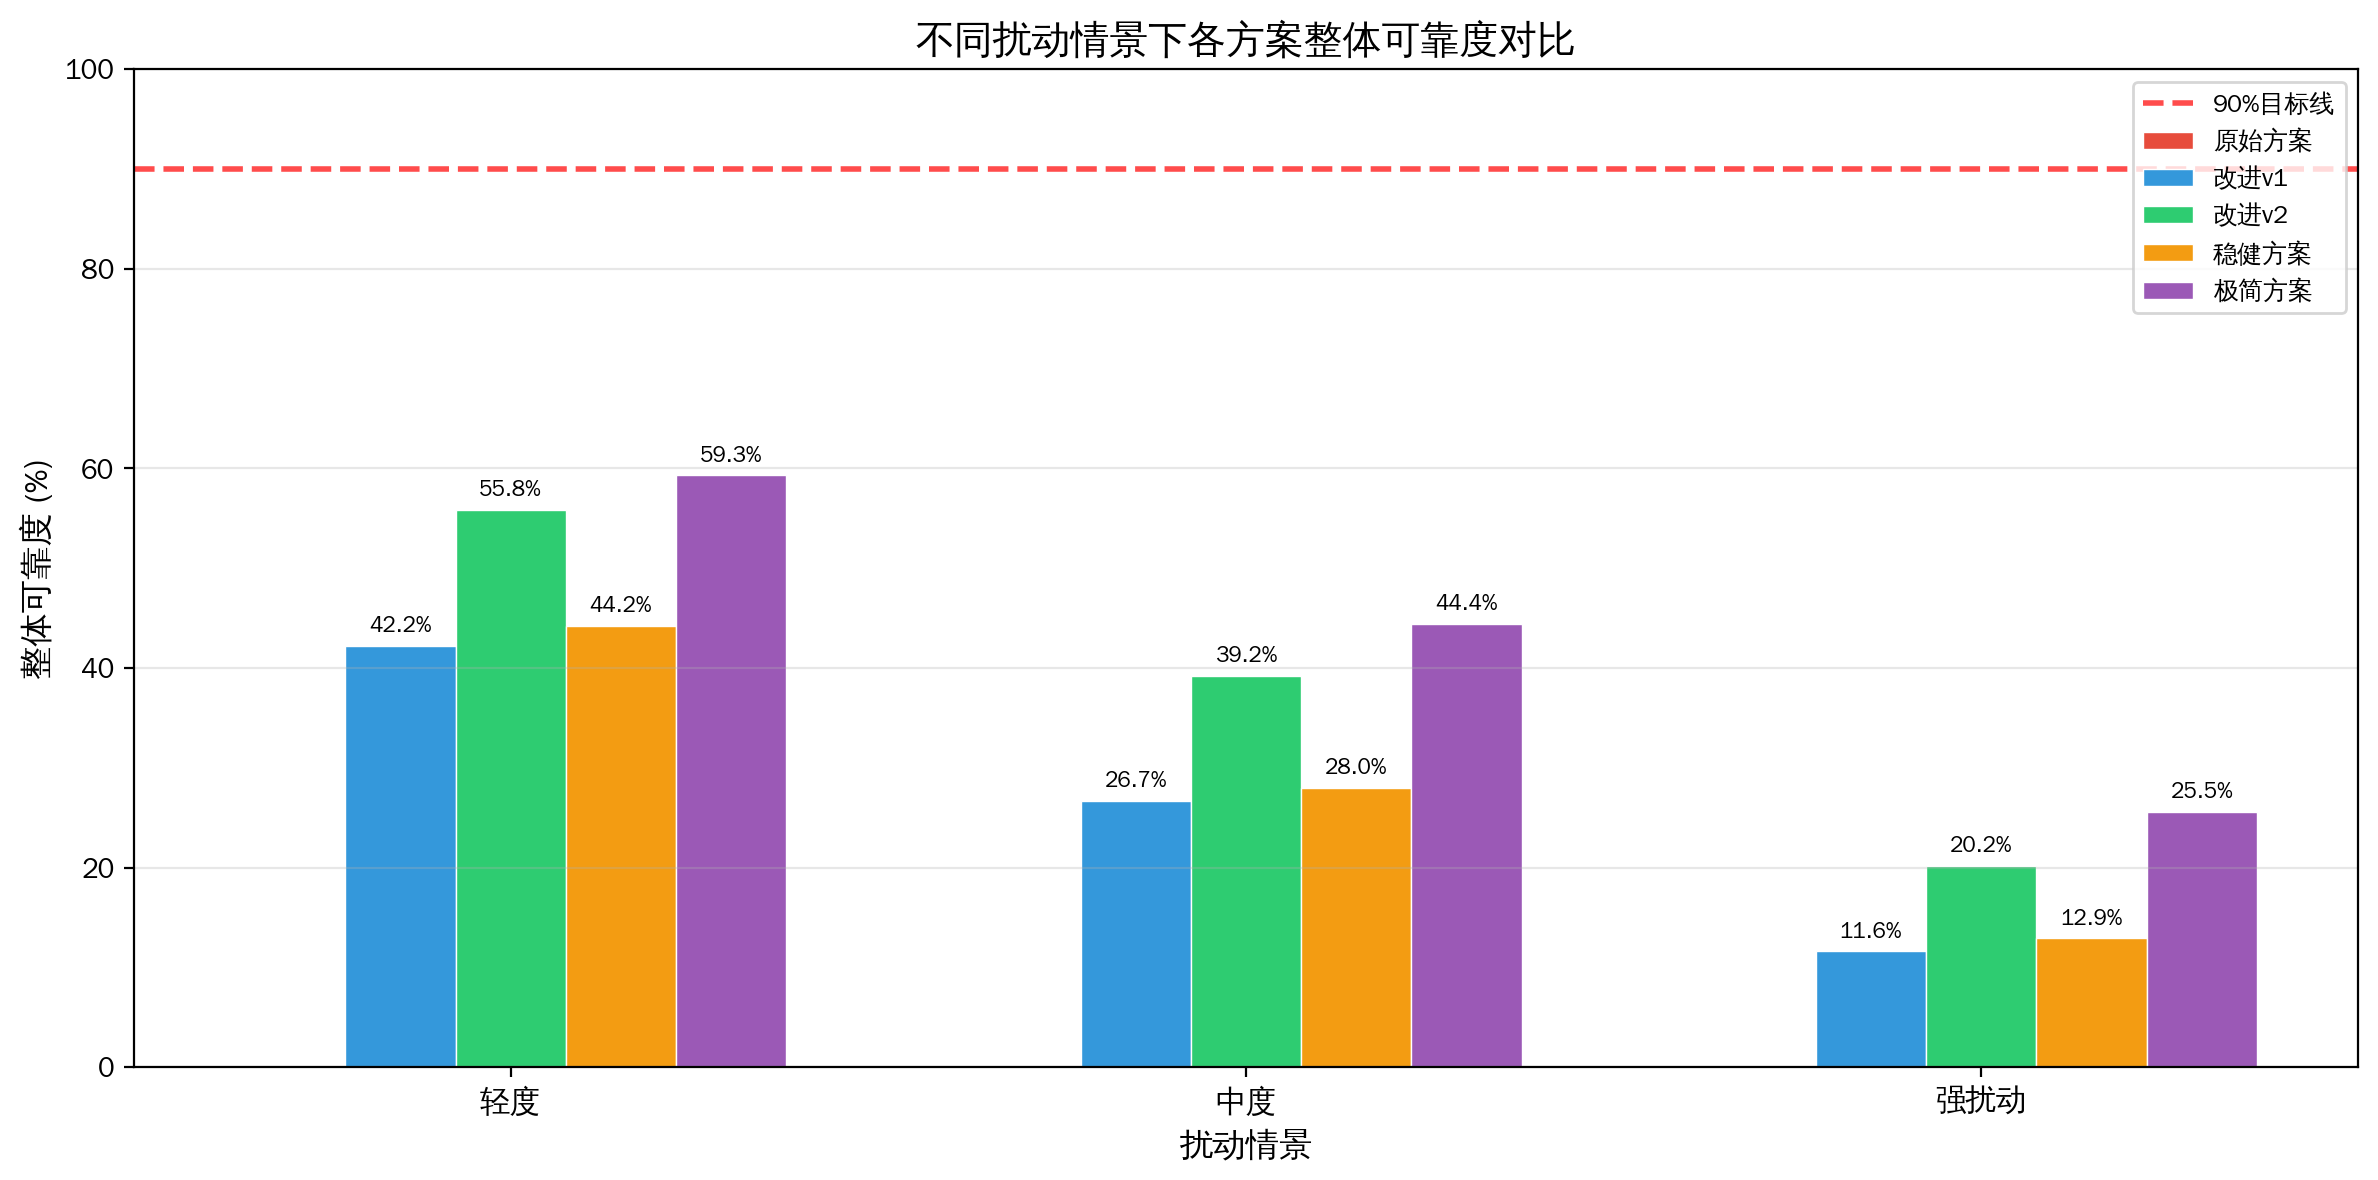
\includegraphics[width=0.82\textwidth]{fig_new_reliability.png}
\caption{不同扰动情景下各方案整体可靠度对比}
\label{fig:newrel}
\end{figure}

由图 \ref{fig:newrel} 可知，在所有扰动情景下，改进方案的可靠度均显著高于原始方案。但需要注意的是，即使改进方案在轻度扰动下可靠度也仅为 55.81\%，仍未达到 90\% 的稳定性要求。

\begin{figure}[H]
\centering
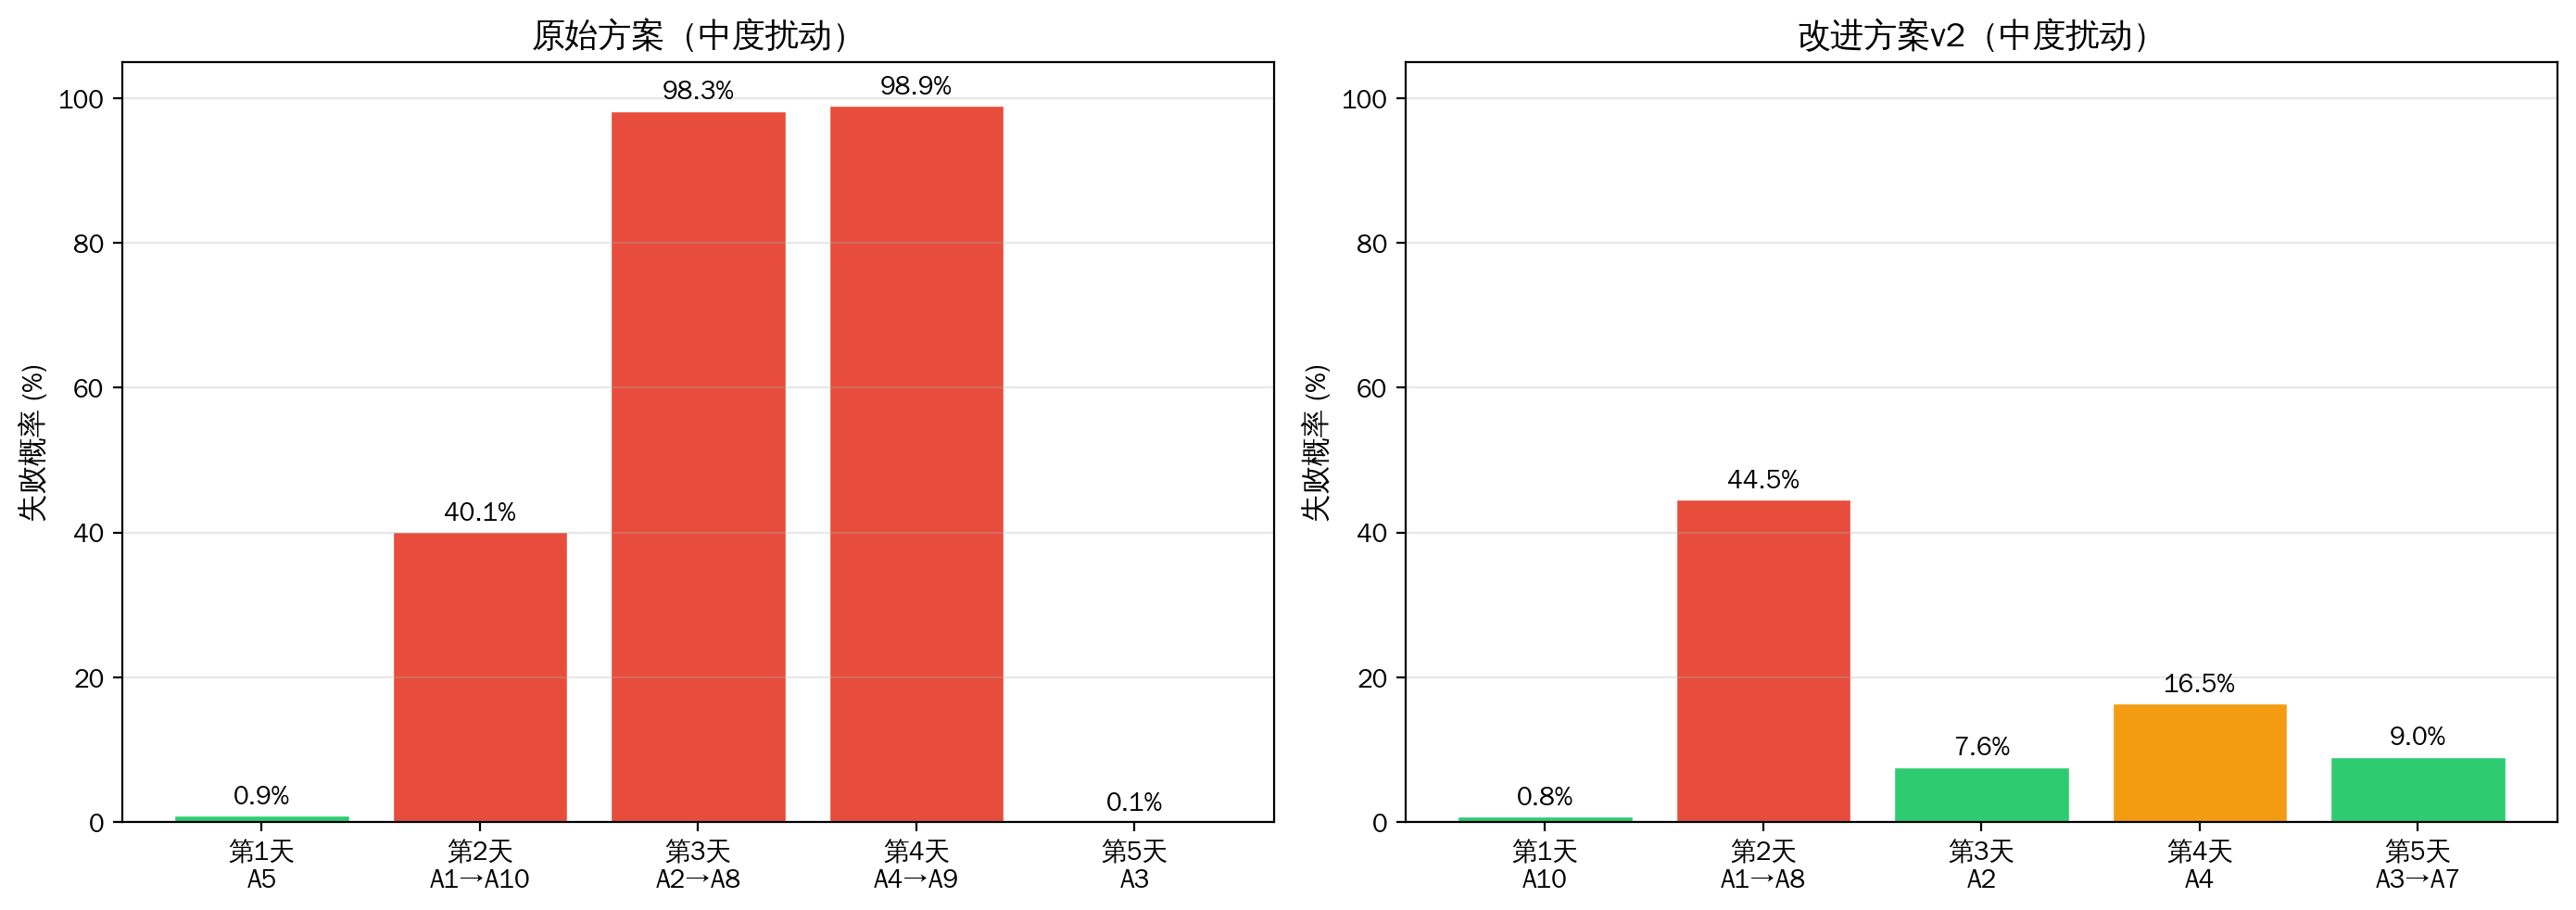
\includegraphics[width=0.85\textwidth]{fig_new_daily_fail.png}
\caption{原始方案与改进方案每日失败概率对比（中度扰动）}
\label{fig:newdaily}
\end{figure}

由图 \ref{fig:newdaily} 可知，改进方案的每日失败概率分布更加均匀，不再出现原始方案中第 3、4 天接近 100\% 失败的极端情况。改进方案的主要薄弱点转移至第 2 天 A1+A10（34.6\%），其原因是该双景点组合仍有一定时间压力。


%% ========== 问题三新增: 灵敏度分析 ==========
\subsection{堵车概率灵敏度分析}

由于题目未明确给出道路拥堵发生概率，本文对高峰拥堵概率 $p_1$ 进行灵敏度分析。设平峰拥堵概率 $p_2 = 0.4 p_1$，令 $p_1$ 从 0.05 到 0.50 步进变化，分别评估原始方案和改进方案的可靠度，结果如图 \ref{fig:sens} 所示。

\begin{figure}[H]
\centering
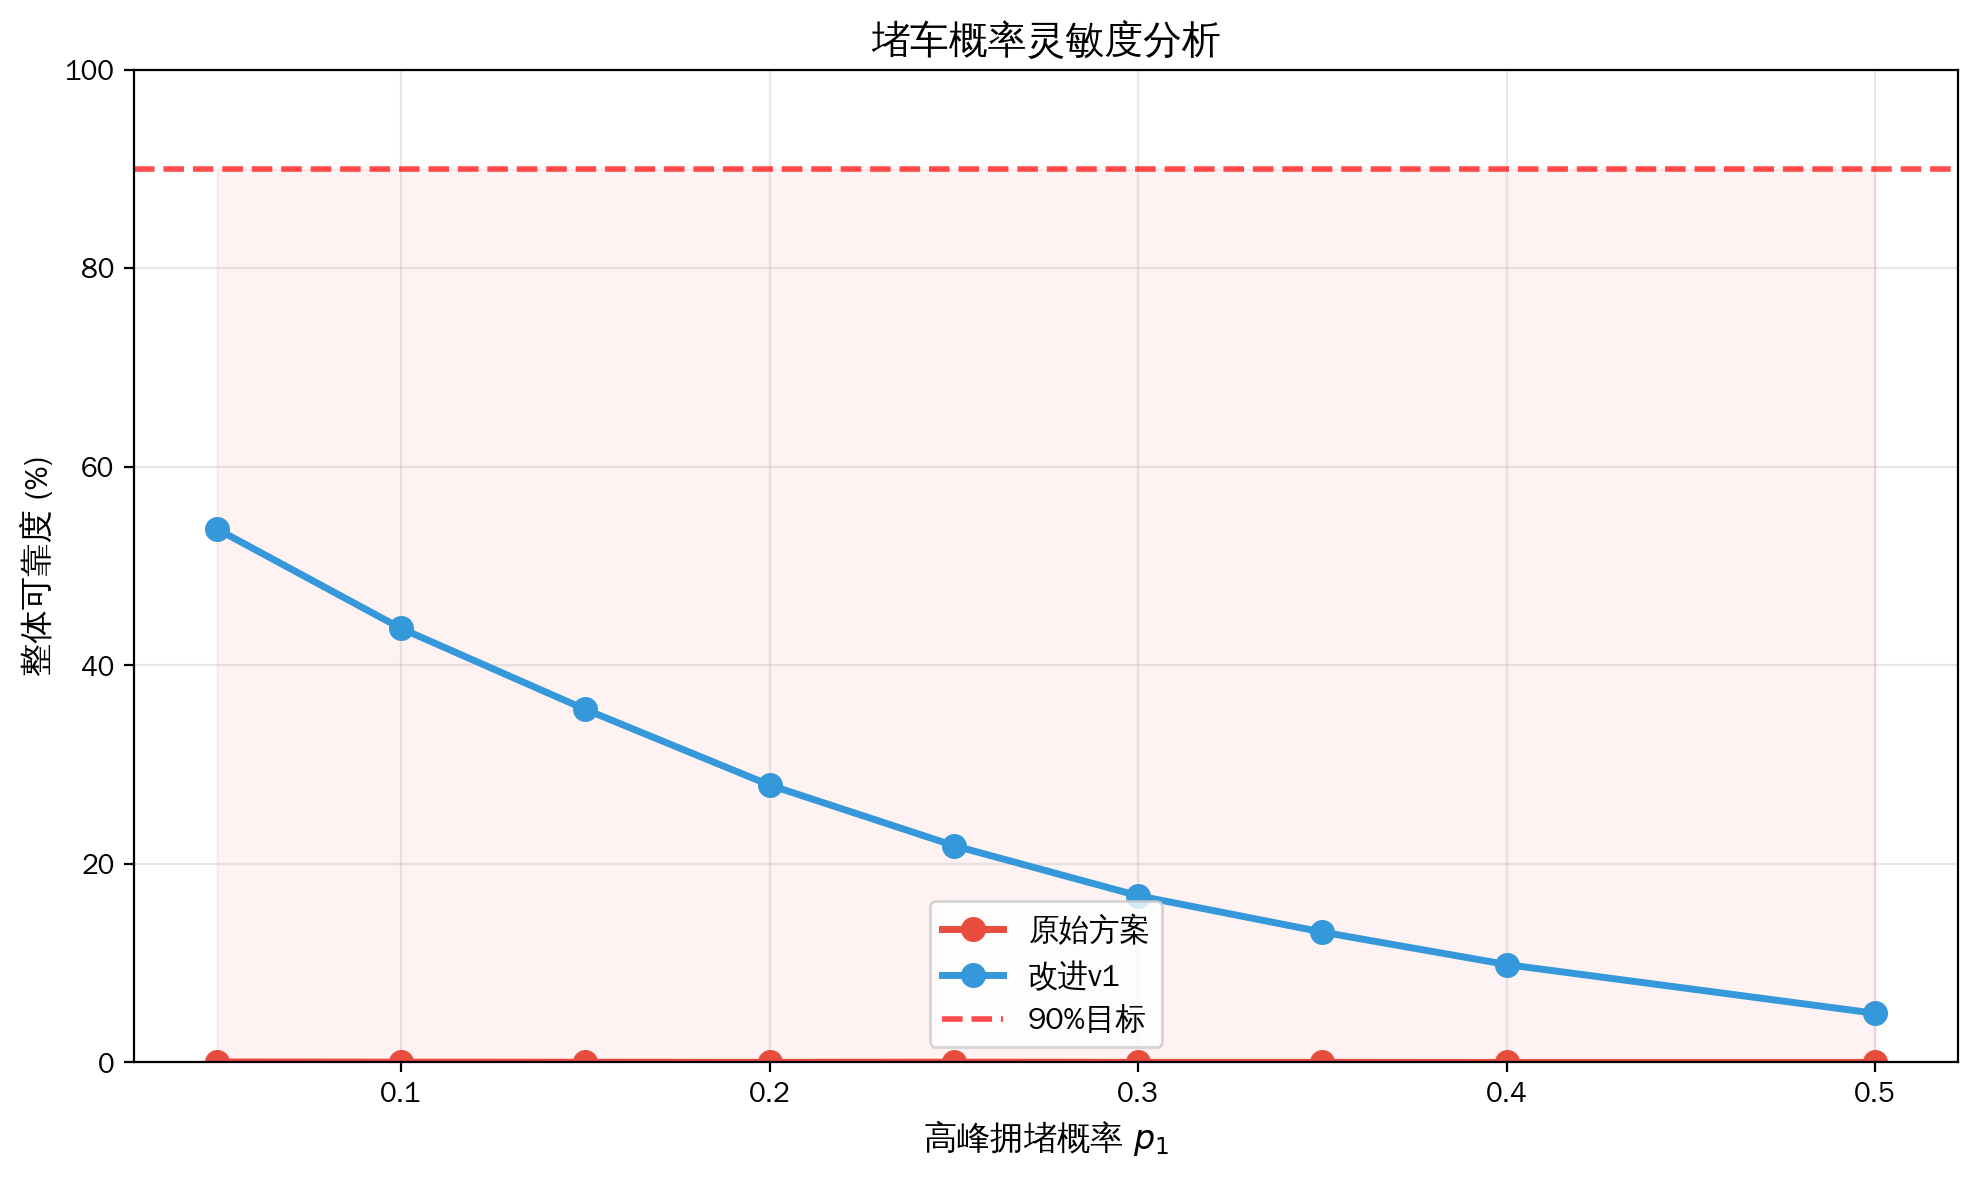
\includegraphics[width=0.78\textwidth]{fig_new_sensitivity.png}
\caption{堵车概率灵敏度分析}
\label{fig:sens}
\end{figure}

由图 \ref{fig:sens} 可知，原始方案在所有堵车概率下可靠度均接近 0\%，说明其不可靠性是结构性的，不依赖于堵车概率假设。改进方案的可靠度随 $p_1$ 增大而下降，从 $p_1=0.05$ 时的 53.7\% 降至 $p_1=0.50$ 时的 5.0\%。即使在最乐观的拥堵假设下，改进方案仍无法达到 90\% 可靠度目标，说明需要进一步减少高负荷景点组合或缩短高耗时景点的游览时间。


%% ========== 问题三新增: Pareto分析 ==========
\subsection{满意度-可靠度 Pareto 分析}

为探索满意度与可靠度之间的权衡关系，本文设计 5 种不同保守程度的行程方案，比较其在中度扰动下的表现，如图 \ref{fig:pareto} 所示。

\begin{figure}[H]
\centering
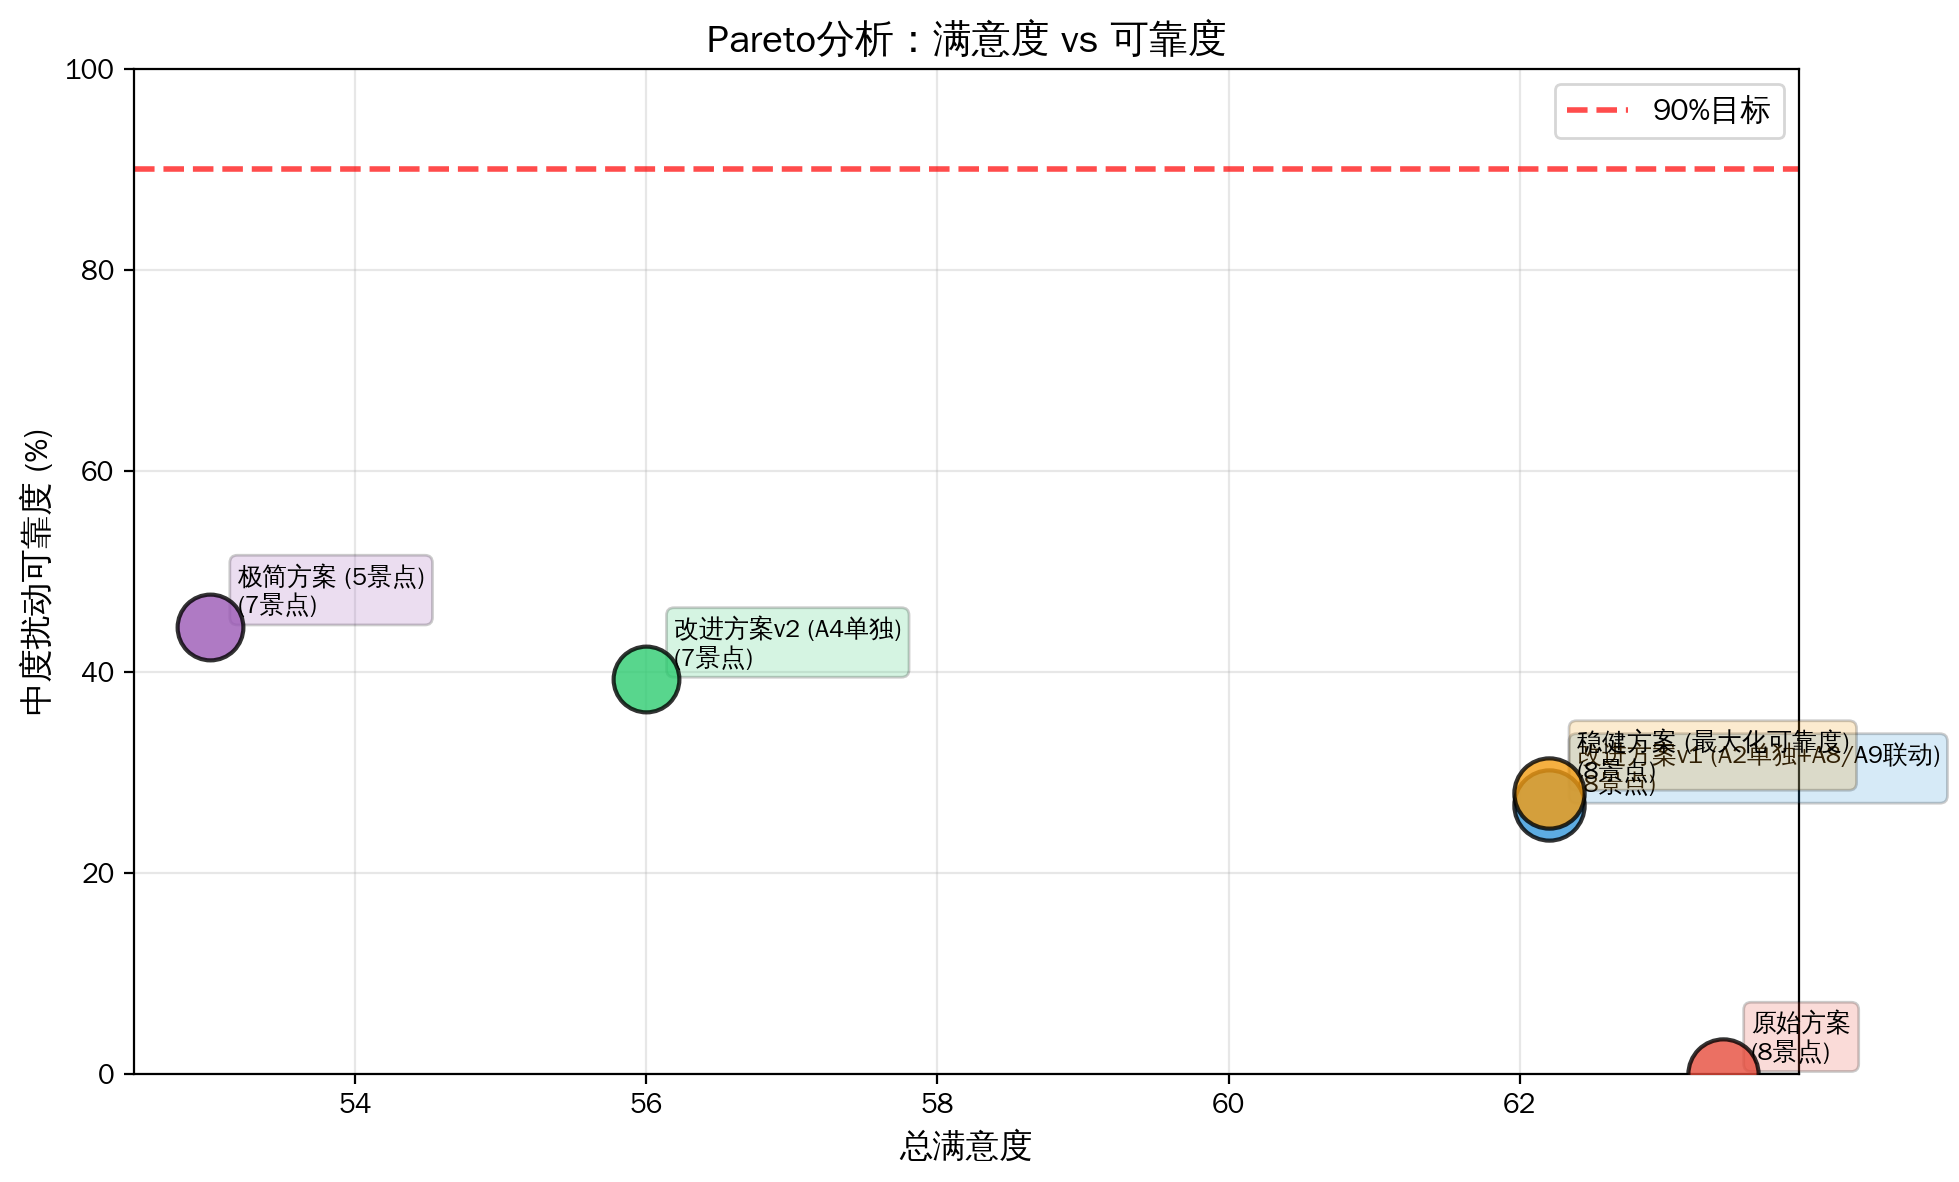
\includegraphics[width=0.78\textwidth]{fig_new_pareto.png}
\caption{满意度-可靠度 Pareto 分析}
\label{fig:pareto}
\end{figure}

由图 \ref{fig:pareto} 可知，满意度与可靠度之间存在明显的负向权衡关系。原始方案追求最大满意度（63.4）但可靠度接近 0\%；极简方案（5 景点）可靠度最高（44.4\%）但满意度最低（53.0）。改进方案位于两者之间，提供了相对均衡的折中。值得注意的是，所有方案均未达到 90\% 可靠度目标线，说明在五一高峰扰动环境下，要同时实现高满意度和高可靠度是一个具有挑战性的多目标优化问题。


%% ========== 问题三修改: 结论 (替换原结论) ==========
\subsection{问题三结论}

通过蒙特卡罗模拟，本文发现原始基准方案在纳入第 1--4 天晚餐后，理想条件下第 3、4 天结束时间已接近 21:00 边界，随机扰动下整体可靠度接近 0\%。这一结果揭示了原始方案的结构性缺陷：高耗时双景点叠加导致时间缓冲被完全消耗。

通过调整每日景点组合，改进方案将第 3、4 天的双景点拆分为单景点，并在第 5 天增加低负荷缓冲景点，中度扰动可靠度从 0.01\% 提升至 39.24\%。灵敏度分析表明，原始方案的不可靠性不依赖于堵车概率假设，是结构性问题。Pareto 分析揭示了满意度与可靠度之间的负向权衡关系。

总体而言，若要求整体可靠度达到 90\% 以上，需要进一步采取以下措施之一：（1）将高耗时景点（如 A2 海洋乐园）的游览时间压缩至舒适游览时长以下；（2）减少总景点数量至 5--6 个，增大每日时间缓冲；（3）引入多套备选行程方案，根据当日实际路况动态调整。


%% ========== 模型评价与改进 (补充内容) ==========
%% 在"模型不足"部分新增第5点:
\item 第二问基准行程未纳入第 1--4 天晚餐，与第三问评估口径不一致，导致第三问可靠度评估结果偏低。改进版已将晚餐纳入第二问基准时序。

%% 在"改进方向"部分新增第6点:
\item 可在第二问中直接嵌入蒙特卡罗可靠度评估，构建"期望可靠度约束下的满意度最大化"模型，避免理想最优与稳健最优之间的冲突。具体而言，将目标函数改为 $\max E[Z]$，约束条件增加 $P_{\rm reliable} \geq 0.9$。
